% !TEX root = main.tex

% Stability Region
\section*{Stability analysis}
We analyze the model problem
\begin{align*}
	\hat{q}_{, t} & = \lambda \hat{q}(t)
\end{align*}
where $\lambda \in \mathbb{C}$ and $\text{Re}(\lambda) < 0$.
\par
We can write the solution at time $t$ using a reverse Taylor expansion i.e.
\begin{align*}
	q(t) & = \Big( 1 - \triangle t q_{, t}(t + \triangle t) + \frac{(\triangle t)^{2}}{2} q_{, t, t}(t + \triangle t) - \frac{(\triangle t)^{3}}{6} q_{, t, t, t}(t + \triangle t) + \hdots \Big) \\
		 & = \Big( 1 - \triangle t \lambda  + \frac{(\triangle t)^{2}}{2} \lambda^{2} - \frac{(\triangle t)^{3}}{6} \lambda^{3} + \hdots \Big) q(t + \triangle t) \\
		 & = \Big( 1 - z  + \frac{1}{2} z^{2} - \frac{1}{6} z^{3} + \hdots \Big) q(t + \triangle t)
\end{align*}
where we have defined $z := \triangle t \lambda$.
We can write the solution at the next time step (denoted $q^{n+1}$) as follows
\begin{align*}
	q^{n+1} & = \Bigg( \frac{1}{1 - z  + \frac{1}{2} z^{2} - \frac{1}{6} z^{3} + \hdots} \Bigg) \, q^{n}
\end{align*}
In order for $q^{n+1}$ to not blow up, we have to ensure that the magnitude of the factor $\Bigg( \frac{1}{1 - z  + \frac{1}{2} z^{2} - \frac{1}{6} z^{3} + \hdots} \Bigg)$ is less than or equal to $1$ i.e. we have to ensure that 
\begin{align*}
	\left\lvert \Bigg( \frac{1}{1 - z  + \frac{1}{2} z^{2} - \frac{1}{6} z^{3} + \hdots} \Bigg) \right\rvert  \leq 1 
\end{align*}
or equivalently,
\begin{align*}
	\left\lvert \Bigg( 1 - z  + \frac{1}{2} z^{2} - \frac{1}{6} z^{3} + \hdots \Bigg) \right\rvert \geq 1
\end{align*}
From earlier, we are working with the semi-discrete form of the advection equation
\begin{align*}
	\frac{\partial}{\partial t} \hat{q} & = \mat{D_{N}} \, \vec{\hat{Q}}
\end{align*} 
We had been using reverse Taylor expansions to compute approximate solution values at the $(n+1)^{th}$ time step i.e.
\begin{align*}
	\vec{\hat{Q}}^{n+1} & = \Bigg( \mat{I} + \triangle t \mat{D_{N}} 
										   + \frac{(\triangle t)^{2}}{2} \mat{D_{N}}^{2} 
										   + \frac{(\triangle t)^{3}}{6} \mat{D_{N}}^{3}
										   + \hdots \Bigg)^{-1} \vec{\hat{Q}}^{n}
\end{align*}
where we truncate the matrix before we invert it for computational purposes i.e. the first order implicit method corresponds to multiplication with $\Bigg( \mat{I} + \triangle t \mat{D_{N}} \Bigg)^{-1}$, the second order implicit method corresponds to multiplication with $\Bigg( \mat{I} + \triangle t \mat{D_{N}} + \frac{(\triangle t)^{2}}{2} \mat{D_{N}}^{2} \Bigg)^{-1}$, and so forth.
\par 
Within our code, we noticed first order, second order, and third order convergence rates with the corresponding methods, but the fourth, fifth, and sixth order implicit methods did not converge as expected. 
This is due to the fact that the fourth, fifth, and sixth order methods are not A-stable, as seen by looking at their stability plots.
\begin{figure}[H]
	\centering
	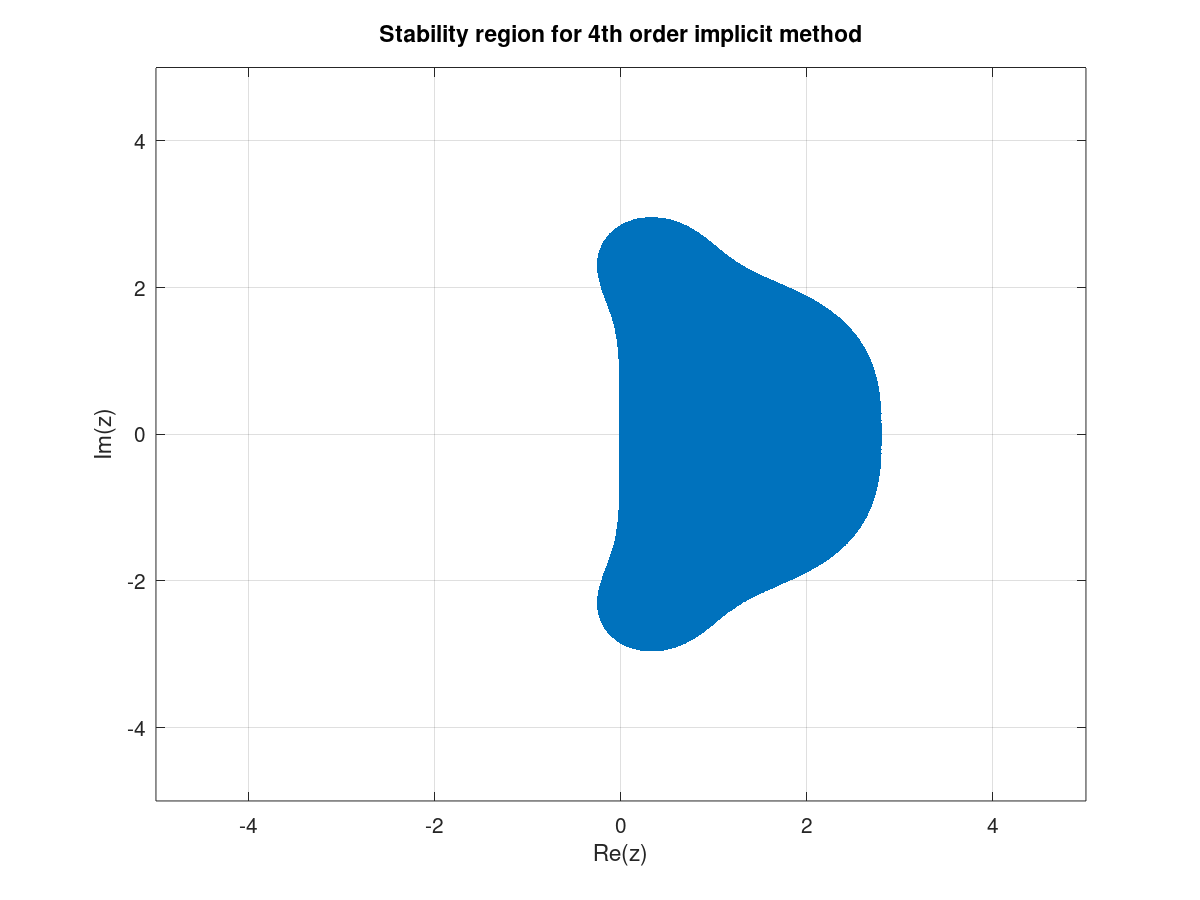
\includegraphics[width=0.75\textwidth]{fourth_order_stab_region.png}
\end{figure}

\begin{figure}[H]
	\centering
	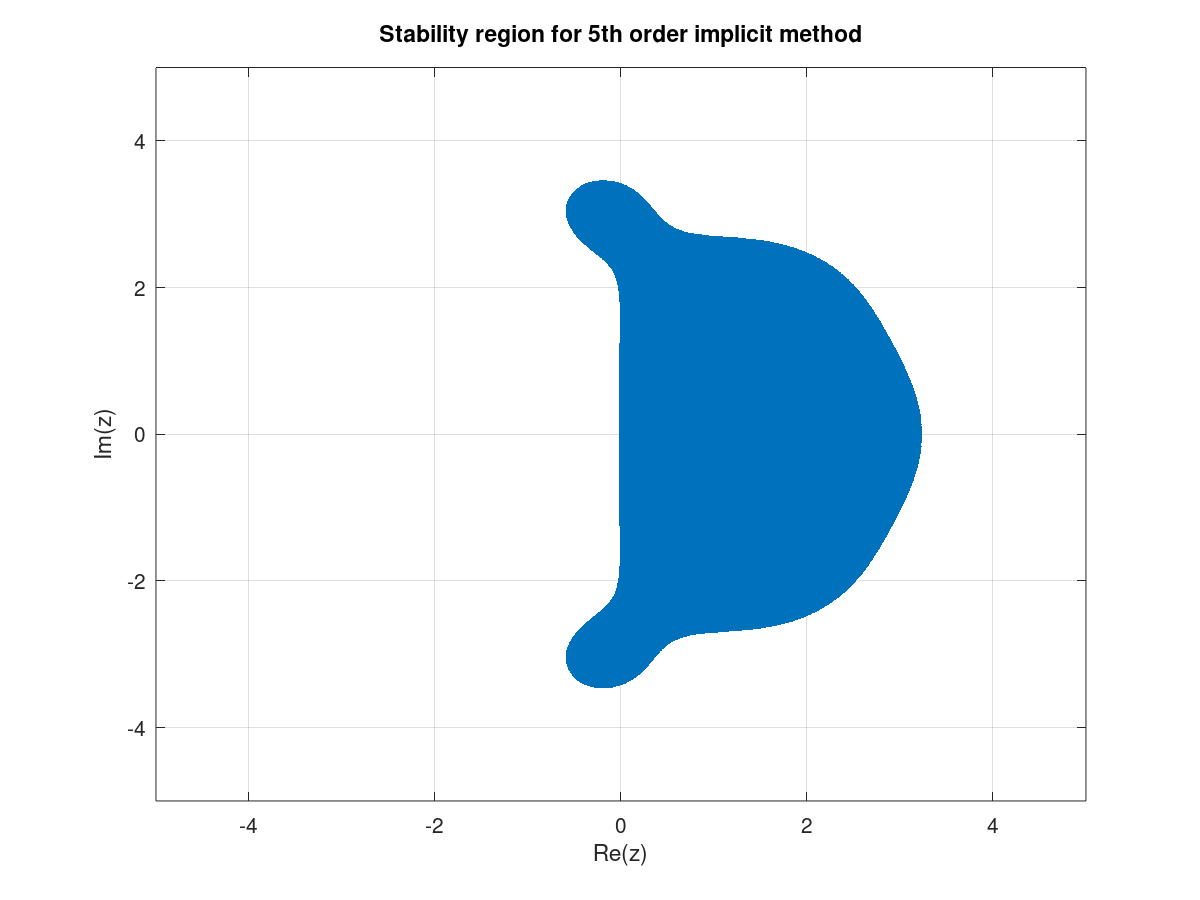
\includegraphics[width=0.75\textwidth]{fifth_order_stab_region.png}
\end{figure}

\begin{figure}[H]
	\centering
	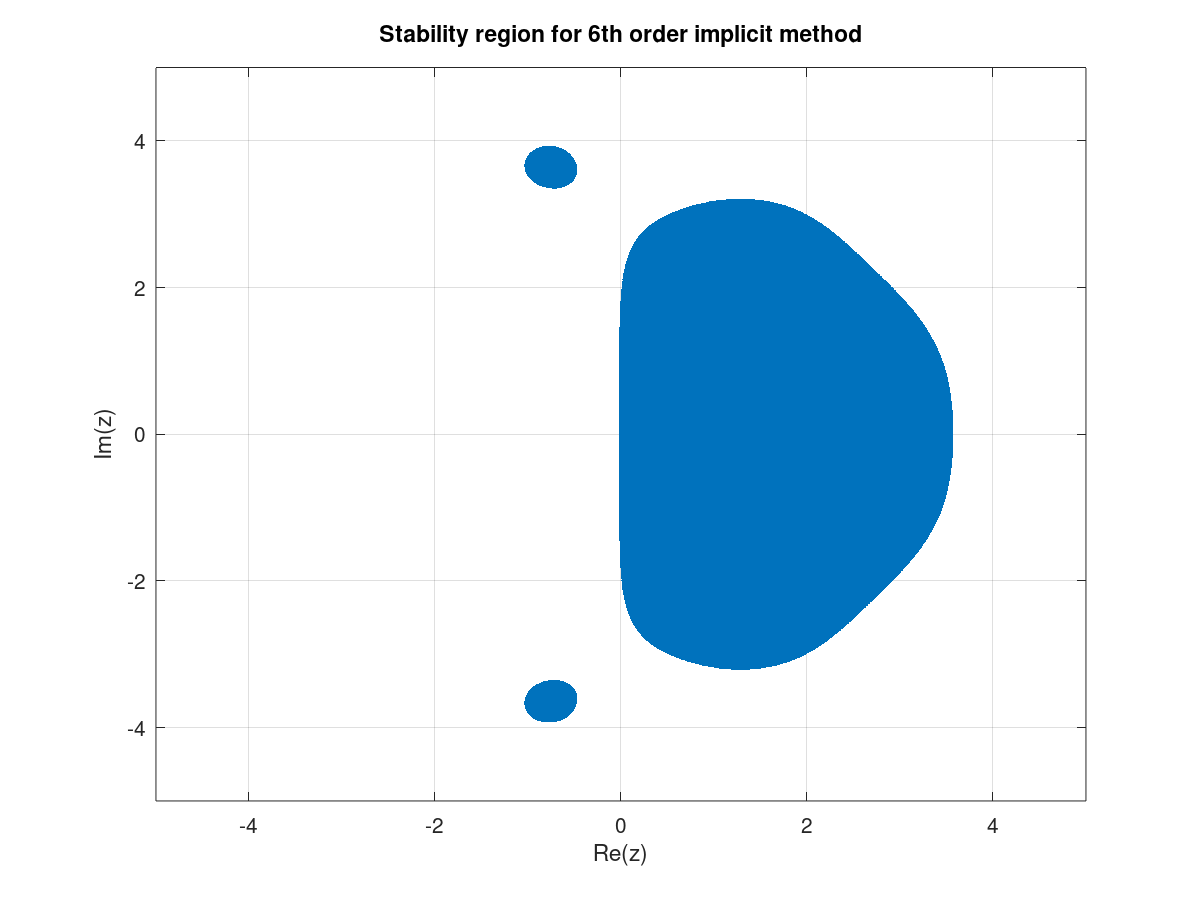
\includegraphics[width=0.75\textwidth]{sixth_order_stab_region.png}
\end{figure}
Because of this, we decided to use backward Euler method as our first order implicit method and the trapezoidal rule as our second order implicit method. 

\section*{New fourth-order time stepping method}
Later in the day, Dr. Rossmanith found a fourth order implicit method that is an extension of the trapezoidal rule. 
\par 
Suppose that our ODE is given by
\begin{align*}
	q_{, t}(t) & = f(t, q(t))
\end{align*}
with the appropriate initial conditions and boundary conditions.
The fourth-order scheme is given by
\begin{align*}
	q^{n+1} = q^{n} + \frac{\triangle t}{2} \Bigg( q_{, t}^{n} + q_{, t}^{n + 1} \Bigg)
					+ \frac{(\triangle t)^{2}}{12} \Bigg( q_{, t, t}^{n} - q_{, t, t}^{n + 1} \Bigg)
\end{align*}
The stability region of the trapezoidal rule is the entire left half of the complex plane.
The stability region of the above rule is also the entire left half of the complex plane.
\par 
We also discussed different time-stepping schemes.
If we assume our ODE is given by
\begin{align*}
	q_{, t}(t) & = f(q(t))
\end{align*}
the second order explicit Runge-Kutta method is given by 
\begin{align*}
	q^{*} & = q^{n} + \triangle t f(q^{n}) \\
	q^{n+1} & = q^{n} + \frac{\triangle t}{2} \Big( f(q^{*}) + f(q^{n}) \Big) 
\end{align*}
We also discussed the difference between \underline{diagonally implicit Runge-Kutta} (DIRK) and \underline{fully implicit} Runge-Kutta schemes.
Roughly speaking, a DIRK method is of the form
\begin{align*}
	q^{(1)} & = q^{n} + c_{1} \triangle t f(q^{n}, q^{(1)}) \\
	q^{(2)} & = q^{n} + c_{2} \triangle t f(q^{n}, q^{(1)}, q^{(2)}) \\
	q^{(3)} & = q^{n} + c_{3} \triangle t f(q^{n}, q^{(1)}, q^{(2)}, q^{(3)}) \\
	        & \vdots 
\end{align*}
We see each computation is ``implicit" (for example, in order to compute $q^{(1)}$, we need to know information about $q^{(1)}$), but each computation is independent of future computations.
On the other hand, a fully implicit Runge-Kutta method is of the form
\begin{align*}
	q^{(1)} & = q^{n} + c_{1} \triangle t f(q^{n}, q^{(1)}, q^{(2)}, q^{(3)}) \\
	q^{(2)} & = q^{n} + c_{2} \triangle t f(q^{n}, q^{(1)}, q^{(2)}, q^{(3)}) \\
	q^{(3)} & = q^{n} + c_{3} \triangle t f(q^{n}, q^{(1)}, q^{(2)}, q^{(3)}) \\
	        & \vdots
\end{align*}
We see that each update computation is potentially coupled with past and future computations.
Fully implicit Runge-Kutta methods tend to have better have convergence rates than DIRK methods, but these fully implicit methods are harder to implement compared to the DIRK methods due to how tightly coupled the updates are in the fully implicit methods. 